\documentclass[border=10pt]{standalone}
\usepackage[T1]{fontenc}
\usepackage{times}
\usepackage{tikz}
\usetikzlibrary{arrows.meta,positioning}

\begin{document}
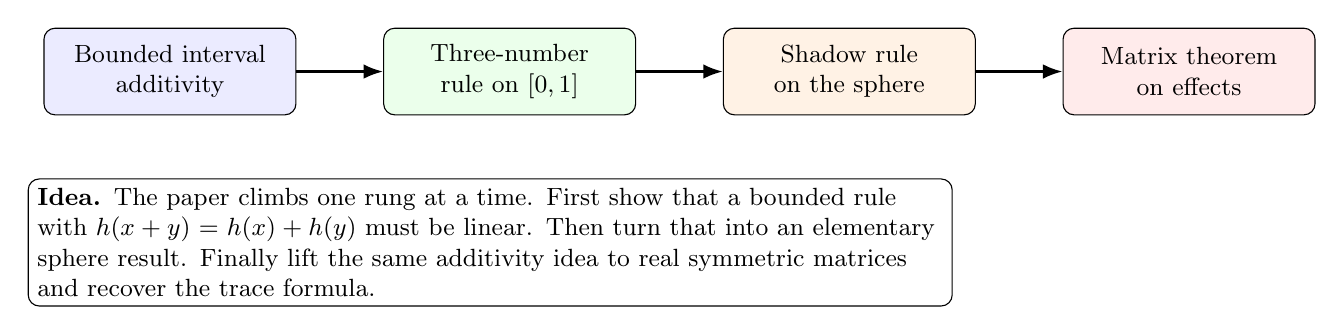
\begin{tikzpicture}[
  >=Latex,
  font=\small,
  box/.style={draw, rounded corners=4pt, align=center, minimum width=3.2cm, minimum height=1.1cm},
  arrow/.style={->, line width=0.9pt}
]
\node[box, fill=blue!8] (a) {Bounded interval\\additivity};
\node[box, fill=green!8, right=1.1cm of a] (b) {Three-number\\rule on $[0,1]$};
\node[box, fill=orange!10, right=1.1cm of b] (c) {Shadow rule\\on the sphere};
\node[box, fill=red!8, right=1.1cm of c] (d) {Matrix theorem\\on effects};

\draw[arrow] (a) -- (b);
\draw[arrow] (b) -- (c);
\draw[arrow] (c) -- (d);

\node[draw, rounded corners=4pt, align=left, fill=white, text width=11.5cm, anchor=north west]
at ([xshift=-0.2cm,yshift=-0.8cm]a.south west) {%
\textbf{Idea.}
The paper climbs one rung at a time.
First show that a bounded rule with $h(x+y)=h(x)+h(y)$ must be linear.
Then turn that into an elementary sphere result.
Finally lift the same additivity idea to real symmetric matrices and recover the trace formula.};
\end{tikzpicture}
\end{document}
